%Version 3.1 December 2024
% Springer Nature sn-jnl template — finalized minimalist Trends & Perspectives draft
% Single illustrative example; curated cites; no undefined macros

\documentclass[pdflatex,sn-mathphys-num]{sn-jnl}

%%%% Standard Packages
\usepackage{graphicx}
\usepackage{multirow}
\usepackage{amsmath,amssymb,amsfonts}
\usepackage{amsthm}
\usepackage{mathrsfs}
\usepackage[title]{appendix}
\usepackage{xcolor}
\usepackage{textcomp}
\usepackage{booktabs}
\usepackage{algorithm}
\usepackage{algorithmicx}
\usepackage{algpseudocode}
\usepackage{listings}

%%%% Theorem Styles (if needed)
\theoremstyle{thmstyleone}
\newtheorem{theorem}{Theorem}
\theoremstyle{thmstyletwo}
\newtheorem{example}{Example}
\newtheorem{remark}{Remark}
\theoremstyle{thmstylethree}
\newtheorem{definition}{Definition}

%%%%%% Planning matrix table stuff
\usepackage{booktabs,tabularx,makecell,array,ragged2e}
\newcolumntype{Y}{>{\RaggedRight\arraybackslash}X} % wrapping, ragged-right body cells
\renewcommand\theadfont{\bfseries}                 % bold headers
\newcommand{\tabitem}{\textbullet\ }               % compact bullet
\newcommand{\cellbullets}[1]{\begin{tabular}[t]{@{}l@{}}#1\end{tabular}}



\raggedbottom

\begin{document}

\allowdisplaybreaks

\title[An Operations Research Agenda for Sustainable Cloud Operations]{An Operations Research Agenda for Sustainable Cloud Operations}

\author*[1]{\fnm{Nathalia} \sur{Wolf}}\email{nathalia.wolf@inria.fr}
\author[1]{\fnm{Luce} \sur{Brotcorne}}
\author[2]{\fnm{Gr\'egory} \sur{Lebourg}}

\affil*[1]{\orgdiv{Univ. Lille, Inria, CNRS, Centrale Lille, UMR 9189 CRIStAL},
  \orgaddress{\street{Parc scientifique de la Haute-Borne, 40 Av. Halley},
  \city{Villeneuve-d'Ascq}, \postcode{59650}, \country{France}}}

\affil[2]{\orgname{OVHcloud},
  \orgaddress{\city{Roubaix}, \country{France}}}

%\abstract{The abstract serves both as a general introduction to the topic and as a brief, non-technical summary of the main results and their implications. Authors are advised to check the author instructions for the journal they are submitting to for word limits and if structural elements like subheadings, citations, or equations are permitted.}
\abstract{
Cloud operations must jointly address cost, performance, and sustainability as data centers scale and energy footprints rise. This paper introduces a planning matrix that organizes cloud and data-center decisions across time horizons (strategic, tactical, operational, real-time) and stages (procurement, production, distribution, sales \& provisioning). 
The matrix provides a structured lens for identifying where Operations Research (OR) models can be developed or extended and how sustainability levers can be integrated. We then instantiate the framework with a illustrative case—\emph{Land \& Building Strategy}. We present the baseline model and subsequently incorporate sustainability-related elements. We conclude with a concise research agenda that highlights modeling patterns and practical opportunities for sustainable cloud operations.
}

\keywords{cloud operations, data centers, operations research, sustainability, planning matrix, facility location}

% Optionally include MSC codes (update as appropriate)
% \pacs[MSC Classification]{90B80, 90C11, 68M20, 90C90}

\maketitle

\section{Introduction}

Cloud computing has reshaped the digital landscape, enabling rapid innovation and scalability. With the global cloud computing market projected to grow from \$371.4 billion in 2020 to over \$832 billion by 2025, reflecting a compound annual growth rate (CAGR) of approximately 17.5\%~\cite{researchmarkets2020}, cloud infrastructures have become the backbone of modern business operations. Public cloud spending alone is expected to reach \$723.4 billion in 2025~\cite{gartner2024}.

In addition to public clouds, private clouds play a crucial role in the modern IT ecosystem. Private clouds refer to dedicated infrastructures—whether on premises or hosted by third parties—tailored to meet the stringent security, compliance, and performance needs of individual organizations. Unlike public cloud services, which are shared among multiple customers, private clouds offer enterprises enhanced control over data and operations.

A major challenge is the increasing complexity of managing large-scale data centers. Rapid growth intensifies concerns around energy consumption, resource allocation, and environmental impact. According to the International Energy Agency, data centers and data transmission networks consumed approximately 260–360 TWh of electricity in 2022, or 1–1.5\% of global electricity use, and were responsible for about 1\% of energy-related greenhouse gas emissions~\cite{iea2023}. Forecasts suggest that data center electricity use could double between 2022 and 2026~\cite{iea2024}, and Goldman Sachs projects that data centers may account for 3–4\% of global electricity demand by 2030, marking a 160\% increase from current levels~\cite{goldman2023}. These trends underscore the dual pressures of maintaining operational efficiency while mitigating environmental impact.

Operations Research (OR) offers a principled set of models and algorithms to address these challenges across time horizons—from long-term strategic planning to real-time execution. The appropriateness of any particular model depends on context, data availability, organizational goals, and constraints; thus, formulations should be seen as templates that can be adapted to specific settings rather than prescriptions. 
 
We propose a planning matrix that organizes cloud and data center decisions by time horizon (strategic, tactical, operational, real-time) and by stage (procurement, production, distribution, sales \& provisioning). The matrix provides a structured lens for identifying decision problems where OR can be applied and how sustainability considerations can be embedded. 
Our contributions are as follows:
\begin{enumerate}
  \item[(i)] A planning matrix for cloud operations that maps decisions across time horizons and stages, offering a structured view of the decision landscape.
  \item[(ii)] A practice-oriented scaffold consisting of the matrix and guiding questions to support modeling and decision support without requiring a full literature survey.
  \item[(iii)] An illustration of use: Land \& Building Strategy (Strategic $\times$ Procurement) formulated as a capacitated facility location model, presented first in a baseline form and then extended with sustainability elements such as carbon and water indicators and latency/coverage constraints.
  \item[(iv)] A concise research agenda summarizing modeling patterns and open OR questions relevant to sustainable cloud operations and industry adoption.
\end{enumerate}

The overall contribution is that the matrix structures a complex activity space and enables a holistic perspective on cloud operations. Establishing such a unified view helps align efforts between academic and industry stakeholders. Comparable planning matrices exist in other domains (e.g., green hydrogen and reverse logistics) \cite{}, and this work adapts the idea to the cloud context.

Having a unified planning matrix is significant because it integrates operational efficiency and environmental stewardship within a single optimization framework. By aligning decision variables and constraints with sustainability objectives—not only cost—this work supports the design of more resilient, efficient, and lower-impact cloud infrastructures.

The remainder of the paper is organized as follows. Section~\ref{sec:methodology} presents the framework based on the planning matrix, alongside guiding questions and sustainability considerations. Section~\ref{sec:example} develops an illustrative case, introducing a baseline model and its sustainability extensions. The paper concludes with a discussion of main findings and directions for future research.


\section{Cloud-operations planning matrix}\label{sec:methodology}

Cloud management involves decisions that range from long term strategic planning to real time execution. Addressing cost, performance, and sustainability across these horizons benefits from a coherent structure. This section adapts the concept of planning matrices from supply chain management to cloud operations. The matrix (i) delineates the decision space and (ii) orients on the formulation of OR models, suggesting how and where sustainability can be embedded.

%Our methodology is built upon three interrelated steps that together provide a comprehensive roadmap for OR practitioners to explore cloud management challenges through the lens of optimization.

\subsection{Scope and dimensions}

The planning matrix is central to our methodology because it provides a systematic framework to categorize and analyze the diverse decision-making challenges inherent in cloud operations. Traditional approaches often focus on individual components or specific time horizons. In contrast, cloud operations are multi-dimensional, involving decisions that span long-term investments, mid-term adjustments, short-term operations, and real-time execution. 
The classic supply-chain planning matrix (see, e.g., \cite{fleischmann2000advanced}) motivates this structure; here it is reinterpreted for cloud operations. Figure~\ref{fig:planning_matrix} illustrates the classic supply chain planning matrix that inspired us. By adapting this framework, we can map each decision-making challenge in cloud operations to a specific time horizon and operational stage, thus providing a structured, comprehensive basis for further formulation of research questions and translation into formal OR problems.

\begin{figure}[h!]
    \centering
    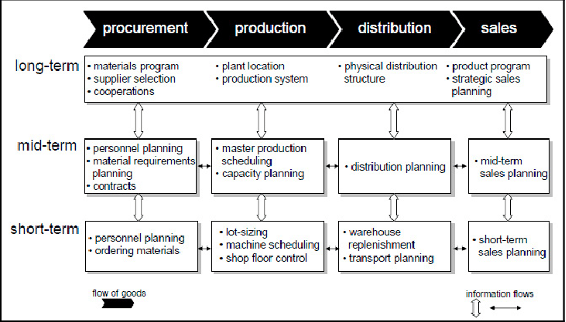
\includegraphics[width=0.7\textwidth]{fig/matrix0.png}
    \caption{Classic supply chain planning matrix \cite{fleischmann2000advanced}}
    \label{fig:planning_matrix}
\end{figure}

A planning matrix offers the following advantages:

\begin{itemize}
    \item \textbf{Comprehensive Coverage:} By mapping decisions across multiple time horizons and operational stages, the matrix ensures that all aspects of management are considered.
    \item \textbf{Structured Analysis:} The matrix facilitates a systematic breakdown of complex problems. This structure helps in identifying specific challenges at each intersection.
    \textbf{Industry Practice:} The matrix utilizes established planning methodologies from supply chain management, modifying them to address cloud operations. %This ensures that the framework remains both rigorous and practical.
    \item \textbf{Integration of Sustainability:} The matrix facilitates the inclusion of sustainability considerations from the outset of decision-making. By organizing problems by horizon and stage, it becomes easier to identify where environmental measures can be embedded.
\end{itemize}

The traditional supply chain matrix focuses on production, inventory, and distribution decisions; our adaptation reinterprets these dimensions for the cloud context, thereby addressing the multifaceted nature of cloud operations. 
Planning matrices have been applied in other domains, such as green hydrogen planning \cite{sgarbossa2023renewable} and reverse logistics \cite{nuss2015reverse}, to structure interdependent decisions across time and functional areas. 
Similarly, our proposed cloud-operations planning matrix provides a systematic way to categorize the diverse decision problems in cloud management. Rather than examining components in isolation, the matrix organizes decisions along two dimensions, time horizon and operational stage.  

\subsubsection{Time horizons}
\begin{itemize}
    \item \textbf{Long-term (Strategic):} Focused on infrastructure planning and major investments, this time horizon encompasses decisions with long-lasting impacts such as data center siting, long-term energy contracts, and major hardware procurement.
    \item \textbf{Mid-term (Tactical):} This level addresses resource allocation and operational strategies that bridge the gap between strategic planning and day-to-day execution, including capacity planning and hardware refresh cycles.
    \item \textbf{Short-term (Operational):} Concerned with real-time execution and dynamic adjustments, this level focuses on immediate actions like workload scheduling, daily maintenance, and reactive procurement during demand surges.
    \item \textbf{Real-time (Execution):} Distinct from short-term operations, this category captures instantaneous responses to unexpected events, such as rapid incident management, real-time monitoring, and immediate adjustments to hardware or network configurations.
\end{itemize}

\subsubsection{Operational stages}
\begin{itemize}
    \item \textbf{Procurement (Hardware and Facilities):} Involves decisions regarding the acquisition of physical assets—servers, cooling systems, data center facilities.
    \item \textbf{Production (Data Center Operations):} Encompasses the day-to-day functioning of data centers, including capacity planning, workload scheduling, and routine maintenance.
    \item \textbf{Distribution (Network and Delivery):} Focuses on the optimization of network resources such as traffic routing, bandwidth management, and content delivery.
    \item \textbf{Sales \& Provisioning (Cloud Services):} Covers customer-facing operations like managing service offerings, pricing strategies, and ensuring compliance with service-level agreements (SLAs).
\end{itemize}


\subsection{The matrix}

Cloud operations involve a wide range of decisions that unfold across different time horizons—from long-term strategic investments (e.g., data center siting) to real-time operational actions (e.g., dynamic workload scheduling). 
The planning matrix provides a structured way to organize these decisions, identify where optimization can add value and how sustainability measures can be incorporated from the start. 
Table~\ref{tab:cloud-planning-matrix} presents the proposed matrix, positioning representative decision classes according to their time horizon and operational stage.

\begin{table*}[h!]
\caption{Cloud planning matrix}
\label{tab:cloud-planning-matrix}
    \centering
    \renewcommand{\arraystretch}{1.3}
    \resizebox{1\textwidth}{!}{%
    \begin{tabular}{@{}p{3cm} p{6cm} p{6cm} p{6cm} p{6cm}@{}}
        \toprule
        \textbf{Time Horizon} & 
        \textbf{Procurement\newline(Hardware, Facilities)} & 
        \textbf{Production\newline(Data Center Ops)} & 
        \textbf{Distribution\newline(Network \& Delivery)} & 
        \textbf{Sales \& Provisioning\newline(Services)} \\
        \midrule
        
        \parbox[c]{3cm}{\centering \textbf{Long-Term}\newline\textit{(Strategic)}} 
        & \begin{minipage}[t]{6cm} \raggedright
            \textbullet\ \textcolor{black}{Land \& building strategy}\newline
            \textbullet\ \textcolor{black}{Plant design}\newline
            \textbullet\ \textcolor{black}{Energy mix selection}\newline
            \textbullet\ \textcolor{black}{Long-term vendor selection}
        \end{minipage} 
        & \begin{minipage}[t]{6cm} \raggedright
            \textbullet\ Capacity planning\newline
            \textbullet\ Technology roadmap
        \end{minipage} 
        & \begin{minipage}[t]{6cm} \raggedright
            \textbullet\ Global network design \newline
            \textbullet\ Edge/PoP placement \newline
            \textbullet\ Interconnect strategy 
        \end{minipage} 
        & \begin{minipage}[t]{6cm} \raggedright
            \textbullet\ Service portfolio definition 
        \end{minipage} \\
        \midrule
        
        \parbox[c]{3cm}{\centering \textbf{Mid-Term}\newline\textit{(Tactical)}} 
        & \begin{minipage}[t]{6cm} \raggedright
            \textbullet\ Hardware upgrade scheduling \newline %refresh/
            \textbullet\ Contract negotiation \newline %renewal/
            \textbullet\ Budget allocation 
        \end{minipage} 
        & \begin{minipage}[t]{6cm} \raggedright
            \textbullet\ Resource capacity allocation \newline
            \textbullet\ Data center consolidation \newline
            \textbullet\ Automation \& orchestration rollout 
        \end{minipage} 
        & \begin{minipage}[t]{6cm} \raggedright
            \textbullet\ Bandwidth scalability \newline
            \textbullet\ Peering adjustment \newline
            \textbullet\ Transport/logistics 
        \end{minipage} 
        & \begin{minipage}[t]{6cm} \raggedright
            \textbullet\ Pricing \& promotion \newline
            \textbullet\ New service introduction/retirement 
        \end{minipage} \\
        \midrule
        
        \parbox[c]{3cm}{\centering \textbf{Short-Term}\newline\textit{(Operational)}} 
        & \begin{minipage}[t]{6cm} \raggedright
            \textbullet\ Procurement/ordering \newline %Immediate
            \textbullet\ Incident procurement \newline
            \textbullet\ Consumables inventory control 
        \end{minipage} 
        & \begin{minipage}[t]{6cm} \raggedright
            \textbullet\ Workload scheduling \newline %provisioning
            \textbullet\ Monitoring \& maintenance \newline
            \textbullet\ Security patching 
        \end{minipage} 
        & \begin{minipage}[t]{6cm} \raggedright
            \textbullet\ Traffic management/routing \newline
            \textbullet\ Network troubleshooting \newline
            \textbullet\ Edge node adjustment 
        \end{minipage} 
        & \begin{minipage}[t]{6cm} \raggedright
            \textbullet\ Onboarding \& staffing \newline
            \textbullet\ Service adjustment 
        \end{minipage} \\
        \midrule
        
        \parbox[c]{3cm}{\centering \textbf{Real-Time}\newline\textit{(Execution)}} 
        & \begin{minipage}[t]{6cm} \raggedright
            \textbullet\ Inbound delivery coordination 
        \end{minipage} 
        & \begin{minipage}[t]{6cm} \raggedright
            \textbullet\ Live server \& rack operation \newline
            \textbullet\ On-site repair/replacement \newline
            \textbullet\ Live cooling \& power %operation 
        \end{minipage} 
        & \begin{minipage}[t]{6cm} \raggedright
            \textbullet\ Live network adjustment \newline
            \textbullet\ Technician dispatch
        \end{minipage} 
        & \begin{minipage}[t]{6cm} \raggedright
            \textbullet\ Immediate provisioning 
        \end{minipage} \\
        \bottomrule
    \end{tabular}%
    }
\end{table*}

By adopting this planning matrix, we can systematically dissect the cloud operations landscape, ensuring that each decision-making challenge is addressed in a comprehensive and sustainable manner.
Section~\ref{sec:example} discusses in more detail the decisions highlighted in blue within the matrix. 
Appendix~\ref{app:questions} compiles detailed question lists for all decision areas, since a full analysis on every decision exceeds the scope of this thesis.

\subsection{Decision-to-model mapping}

Each decision in the planning matrix can be translated into an optimization model by linking managerial questions to classical OR formulations. The process connects decision drivers and constraints with representative problem classes, such as facility location or scheduling, and incorporates sustainability through objectives, constraints, or incentives. This provides a coherent way to express cloud management challenges as solvable models that capture both performance and environmental goals.


\subsubsection{Key questions.}
%We begin by formulating key guiding questions that frame the decision-making challenge. These questions are derived from real-world concerns in cloud infrastructure and services management and are designed to capture both operational complexity and sustainability goals.
Start by identifying the main drivers and constraints of the decision. Relevant aspects include the goal of the decision, such as reducing cost, improving latency, or increasing availability. Consider the surrounding market and technical environment, including energy prices, incentives, grid mix, climate, and supply risks. Also review the scope of services and demand, the relation with existing assets, possible overlap or cannibalization, and any physical or regulatory requirements such as land, power, water, and permits. Connectivity and resilience are also central, covering redundancy and geographic diversity. These elements define the requirements, trade-offs, and performance indicators that the model must capture.

\subsubsection{Model class selection.}

Each planning decision identified in the matrix can be associated with a representative classical OR problem, such as facility location, capacity planning, job scheduling, project scheduling, portfolio optimization, etc.  
In addition, review general trends in those class of problems and how they have been applied in cloud and data-center settings. Summarize representative references to situate the formulation and indicate whether the class is mature in cloud applications or presents a gap. Consider that proposed OR models are illustrative rather than prescriptive, intended to provide a clear example of how each decision could be approached using OR techniques. 

\subsubsection{OR model formulation.}
Formulating the OR model means translating the decision context into sets, parameters, and decision variables that capture the relevant system dynamics. Constraints encode requirements such as demand satisfaction, service-level agreements, capacity limits, or policy restrictions, while the objective reflects the primary performance measure of interest, e.g., cost, resilience, efficiency, or sustainability.  
In practice, the appropriate formulation depends on several factors:
\begin{itemize} 
    \item the specific context and constraints of the decision,
    \item available data and the dynamics of the system,
    \item the complexity and uncertainty involved,
    \item the decision-maker’s goals, such as cost efficiency, resilience, or sustainability.
\end{itemize}
The result is a baseline model tailored to the decision’s horizon and stage, designed to be tractable yet adaptable to future refinements.


\subsubsection{Sustainability considerations.}

For each planning decision, we also outline how sustainability dimensions—such as energy efficiency, carbon emissions, water usage, and resource circularity—could be incorporated into the OR modeling framework. Rather than providing detailed mathematical formulations, we indicate practical ways to integrate sustainability considerations, typically by:
\begin{itemize}
    \item including sustainability criteria as additional objectives or weighted components within the objective function,
    \item introducing constraints or thresholds to exclude unsustainable options explicitly,
    \item applying penalties or incentives to encourage more environmentally sustainable choices.
\end{itemize}

This decision-to-model procedure provides a consistent path from managerial questions to solvable optimization models, with sustainability integrated by design. 

\section{Application to Land \& Building Strategy} \label{sec:example}
section{Application to Land \& Building Strategy} 

\subsection{Key questions.}

Land \& building strategy decisions focuses on selecting optimal locations for new data centers by evaluating factors such as power costs, local climate, tax policies, and latency requirements.
An operator considers candidate locations for new data centers over a multi-year horizon. Drivers include power availability and price, climate and cooling potential, tax and policy incentives, latency to markets, backbone connectivity, disaster risk, and sustainability goals. 
Key performance indicators (KPIs) include total cost of ownership, latency/service reach, grid- and site-level carbon intensity (operational footprint), water use (cooling and generation), and resilience (e.g., risk of simultaneous outages).

These considerations can be translated into the following questions that cloud decision makers need to ask when deciding on a land \& building strategy for new data centers:
\begin{itemize}
    \item \emph{Rationale:} Why open a data center in a given location? Is it driven by data residency requirements, latency constraints, or market signals indicating rising demand?
    \item \emph{Market Conditions:} Are local market conditions—such as competitive energy costs, low-carbon energy availability, or tax incentives—favorable?
    \item \emph{Climate:} Do climate conditions (e.g., cooler temperatures for natural cooling) contribute to the decision?
    \item \emph{Target Market:} What is the targeted market for the new data center?
    \item \emph{Service Offering:} Which services will be offered initially and over time, and what pricing strategy should be adopted?
    \item \emph{Cannibalization Risk:} How might the new facility impact existing services (e.g., risk of cannibalization)?
    \item \emph{Physical Requirements:} What are the physical requirements (e.g., building and plot size in m\textsuperscript{2}, power draw in MW, water availability in m\textsuperscript{3})?
    \item \emph{Connectivity:} What connectivity requirements exist, and how will the site connect to the network backbone (including cost implications for dark fiber)?
    \item \emph{Standards:} Which data center standard (Tier I–IV) is targeted?
\end{itemize}


\subsection{Model class selection.}

The land \& building strategy decision can be modeled as a \textit{Facility Location Problem} (FLP). 
Facility location models are traditionally designed to determine the number and locations of facilities, their capacities, and the rules for allocating demand to these facilities for service \cite{church2018location,drezner1995survey,drezner2002facility,eiselt2004decision,eiselt2011foundations,eiselt2015applications,farahani2009facility,farahani2019urban}. Some of the trends of FLP include:

\begin{itemize}
    \item \emph{Dynamic Decisions:} Facility location decisions should be reappraised periodically to adapt to a rapidly changing operating environment—leading to dynamic or multi-period facility location models \cite{arabani2012facility}.
    \item \emph{Uncertainty Parameters:} Given the inherent uncertainty in long-term models, frameworks such as stochastic programming, fuzzy programming, and robust optimization are employed to manage risk \cite{correia2015uncertainty,snyder2006facility}.
    \item \emph{Multi-criterion Decisions:} Facility location is influenced by multiple criteria and stakeholder objectives, necessitating multi-criteria optimization approaches \cite{farahani2010multiple}.
    \item \emph{Decision-making Behavior Modeling:} The modeling of decision-makers’ behavior (e.g., through the multinomial logit model and other discrete choice methods) is crucial to capture the impact of individual and group judgment on facility location \cite{mcfadden1974conditional,haase2014comparison,mogale2018bounded}.
    \item \emph{Routing Problem Considerations:} Facility location decisions are often coupled with routing problems—such as the shortest path, TSP, and VRP—resulting in integrated formulations like the location-routing problem (LRP) and location-arc problem (LARP) \cite{daskin2013network}.
    \item \emph{Network-Facility Interaction:} The optimal location of facilities is strongly influenced by network topology. It is important to simultaneously determine network configuration and facility locations, although this interaction remains relatively underexplored \cite{peeters1995effect,daskin2003location}.
\end{itemize}

%%%%PARAGRAPH ON THE RELATIONSHIP, EQUIVALENTE AND MATCH OF THE CLOUD DECISION WITH THE OR PROBLEM

For land and building for cloud computing, potential data center sites are evaluated based on their overall cost-effectiveness and ability to meet key requirements. The goal is to select sites that minimize total costs---covering both the fixed expenses of site development and the ongoing operational costs---while also considering factors such as capacity, connectivity, and performance standards. %Modern facility location models often extend this approach to handle multiple objectives simultaneously, balancing cost considerations with sustainability goals. Essentially, the qualitative key questions regarding market conditions, physical requirements, and connectivity are translated into the criteria and constraints of the model, ensuring that the decision-making process is both systematic and aligned with strategic priorities.
Recent applied research on data center facility location highlights the integration of optimization and real-world considerations such as sustainability, network latency, and resilience. \cite{Wang2023} developed a bi-objective MILP model to jointly minimize total cost and carbon emissions by incorporating site-specific configurations of scale, power source, and cooling technologies. \cite{Liu2023} formulated a high-availability placement model that optimizes primary and backup data center sites in emerging economies, addressing constraints like limited technical workforce and infrastructure reliability. \cite{Vieira2022} studied a hierarchical load distribution model between edge and core data centers under latency constraints, introducing a MILP-based allocation model enhanced with heuristics. In a complementary direction,\cite{Yuna2020} applied a fuzzy multi-criteria decision-making (MCDM) approach to evaluate all 81 provinces of Turkey, considering factors such as disaster risk, energy stability, labor, and climate. These studies collectively demonstrate that modern facility location problems for cloud infrastructure increasingly adopt hybrid models combining MILP, heuristics, and decision support systems to address multi-objective and region-specific challenges.

\subsection{OR model formulation.} 

We present a capacitated facility location with assignment to demand regions and latency-eligibility sets. Let $I$ be the candidate sites and $R$ the demand regions.

For each candidate site $i \in I$, $F_i$ denotes the fixed cost required to open and build out site $i$ (e.g., land, construction, interconnection). The term $O_i$ is the annualized operating cost incurred if site $i$ is opened (e.g., energy, staffing, taxes, leases), expressed on the same cost basis as the objective. The quantity $C_i$ is the effective service capacity of site $i$ (for instance, an MW-equivalent, IT power, or a normalized service unit). For each demand region $r \in R$, $d_r$ is the demand that must be served, measured in the same units as $C_i$. The value $c_{ir}$ measures latency or distance from site $i$ to region $r$ and is used both to restrict admissible assignments and (optionally) to penalize longer links in the objective. Given a maximum acceptable latency $L_r^{\max}$ for region $r$, we define the eligibility set
\[
A_r := \{\, i \in I : c_{ir} \le L_r^{\max} \,\},
\]
so that only sites in $A_r$ may serve region $r$. Finally, $\phi \ge 0$ is an optional coefficient converting the latency/distance metric into a cost term; setting $\phi=0$ removes this proxy from the objective.

For each site $i \in I$, the binary variable $x_i \in \{0,1\}$ indicates whether the site is opened ($x_i=1$) or not ($x_i=0$). For each admissible pair $(i,r)$ with $i \in A_r$, the continuous variable $y_{ir} \ge 0$ represents the amount of demand of region $r$ served from site $i$. These flows satisfy regional demand balance and are limited by the capacity of any opened site.

Thus, we will have the following model:
\begin{align}
\min \ \ & \sum_{i \in I} (F_i + O_i) x_i \;+\; \phi \sum_{r \in R}\sum_{i \in A_r} c_{ir}\, y_{ir} \label{eq:base-obj}\\
\text{s.t. } 
& \sum_{i \in A_r} y_{ir} \;=\; d_r \qquad \forall r \in R \label{eq:base-demand}\\
& \sum_{r \in R} y_{ir} \;\le\; C_i\, x_i \qquad \forall i \in I \label{eq:base-capacity}\\
& y_{ir} \;\ge\; 0 \quad \forall r \in R, \ \forall i \in A_r, \qquad x_i \in \{0,1\} \ \forall i \in I. \label{eq:base-bounds}
\end{align}

Extensions can include multi-period opening decisions, uncertainty (robust sets over power prices or grid mix), multi-criteria decision analysis (MCDA) overlays, and integrated location–network co-design when backbone build-outs are endogenous.

\subsection{Sustainability considerations.}

Sustainable site selection plays a crucial role in minimizing the environmental footprint of new data centers. In addition to traditional economic and technical criteria, it is essential to assess each candidate location for its potential to support a renewable energy infrastructure, efficient resource usage, and environmentally friendly building practices. We can consider the following:

\begin{itemize}
  \item {Usage-based environmental caps.}
  Limit total emissions and water use based on actual assignment flows using site-specific factors per unit served:
  \begin{align}
    \sum_{r \in R} \sum_{i \in A_r} e_i^{\mathrm{CO_2}} \, y_{ir} \;\le\; \Gamma_{\mathrm{CO_2}}, 
    \qquad
    \sum_{r \in R} \sum_{i \in A_r} w_i \, y_{ir} \;\le\; \Gamma_{\mathrm{W}}. 
    \label{eq:usage-caps}
  \end{align}
 
  \item {Capacity-based environmental caps.}
  When usage data are not available at the required granularity, cap impacts via capacity-weighted openings as a conservative proxy:
  \begin{align}
    \sum_{i \in I} e_i^{\mathrm{CO_2}} \, C_i \, x_i \;\le\; \bar{\Gamma}_{\mathrm{CO_2}},
    \qquad
    \sum_{i \in I} w_i \, C_i \, x_i \;\le\; \bar{\Gamma}_{\mathrm{W}}.
    \label{eq:capacity-caps}
  \end{align}
 

  \item {Renewable share requirement.}
  Enforce a minimum portfolio renewable share using site-level fractions; capacity-weighted version:
  \begin{align}
    \sum_{i \in I} \rho_i \, C_i \, x_i \;\ge\; \rho_{\min} \sum_{i \in I} C_i \, x_i.
    \label{eq:renewable-share}
  \end{align}
  %(If usage flows are modeled, a usage-weighted variant is \(\sum_{r \in R}\sum_{i \in A_r} \rho_i \, y_{ir} \ge \rho_{\min} \sum_{r \in R}\sum_{i \in A_r} y_{ir}\).)
  To discourage low-renewable sites without forbidding them, add a shortfall penalty to the objective \eqref{eq:base-obj}:
  \begin{align}
    \min \ \cdots \;+\; 
    \lambda_{\mathrm{R}} \sum_{i \in I} \delta_i \, C_i \, x_i,
    \qquad 
    \delta_i := \max\{0,\rho_{\min}-\rho_i\}.
    \label{eq:renewable-penalty}
  \end{align}
 
  
  \item {Objective scalarization.}
  Internalize environmental impacts by augmenting the economic objective \eqref{eq:base-obj}; tuning the weights traces the trade-off frontier:
  \begin{align}
    \min \ \cdots \;+\;
    \lambda_{\mathrm{C}} \sum_{r \in R}\sum_{i \in A_r} e_i^{\mathrm{CO_2}} \, y_{ir}
    \;+\;
    \lambda_{\mathrm{W}} \sum_{r \in R}\sum_{i \in A_r} w_i \, y_{ir}.
    \label{eq:scalarized}
  \end{align}
 

  \item {Minimum efficiency or building standards.}
  Ensure only sufficiently efficient sites can be opened (e.g., via a building-efficiency score \(\eta_i\)) either by prefiltering or via an eligibility parameter \(z_i\in\{0,1\}\) (1 if site \(i\) meets the standard):
  \begin{align}
    x_i \;\le\; z_i \qquad \forall i \in I,
    \label{eq:efficiency-eligibility}
  \end{align}
  or, equivalently, forbid below-threshold sites:
  \begin{align}
    \sum_{i \in I:\ \eta_i < \eta_{\min}} x_i \;=\; 0.
    \label{eq:efficiency-min}
  \end{align}
  To reward higher efficiency, include a credit in the objective \eqref{eq:base-obj}:
  \begin{align}
    \min \ \cdots \;-\; \kappa \sum_{i \in I} \eta_i \, x_i,
    \label{eq:efficiency-credit}
  \end{align}
  where \(\kappa \ge 0\) reflects the internal valuation of efficiency (e.g., expected OPEX savings or incentives).
 
\end{itemize}

\subsection{Numerical analysis}\label{sec:num}

We illustrate the models with a controlled toy instance generated by the functions in \texttt{src/models/cflp.py}. The goal is to show how adding sustainability levers alters siting and allocation choices; we do not attempt geographic calibration. Table~\ref{tab:instance} summarizes the instance: 10 candidate sites, 8 demand regions, total demand of 502.9 units, heterogeneous costs and capacities, and site-specific CO$_2$ and water factors. Latency eligibility is defined by a region-specific 60th-percentile distance threshold and a latency proxy weight $\phi=10$ in the objective.

\begin{table}[t]
  \centering
  \caption{Toy instance definition.}
  \label{tab:instance}
  \input{../results/tables/table1_instance_summary}
\end{table}

Three model variants are solved on this instance. The \emph{baseline} uses \eqref{eq:base-obj}--\eqref{eq:base-bounds} with latency proxy; sustainability is measured ex post. The \emph{capped-impact} model adds usage-based caps \eqref{eq:usage-caps} set at 85\% of the baseline CO$_2$ and water levels ($\Gamma_{\mathrm{CO_2}}=280.9$, $\Gamma_{\mathrm{W}}=106.2$). The \emph{scalarized} model replaces the objective with \eqref{eq:scalarized} and sweeps $(\lambda_{\mathrm{C}},\lambda_{\mathrm{W}})\in\{0,1,5,10,25,50\}^2$ to map cost–impact trade-offs.

\paragraph{Results.} Table~\ref{tab:kpi} reports portfolio KPIs. The baseline opens seven sites (S10,S2,S5,S6,S7,S8,S9) with total cost 3197.7, ex-post CO$_2$ 332.2, and water 139.4. Tightening caps pushes the model to replace S10 with a cleaner site (S4), cut CO$_2$ by 15\% and water by 24\%, at a 4.4\% cost increase; the opened set remains of size seven. Table~\ref{tab:siteshifts} details site-level flow shifts, with the largest reallocation from S10 to S4. The scalarized runs trace a smooth frontier: raising $(\lambda_{\mathrm{C}},\lambda_{\mathrm{W}})$ to (50,50) lowers CO$_2$ to 278.6 and water to 94.9 for a modest cost increase to 3311.9.

\begin{table}[t]
  \centering
  \caption{Baseline vs sustainability-aware KPIs.}
  \label{tab:kpi}
  \input{../results/tables/table2_kpi_comparison}
\end{table}

\begin{table}[t]
  \centering
  \caption{Site-level openings and flow shifts (baseline vs capped-impact).}
  \label{tab:siteshifts}
  \input{../results/tables/table3_site_shifts}
\end{table}

Figure~\ref{fig:maps} shows the siting patterns for baseline and capped-impact runs; eligibility and latency constraints create multiple feasible assignments, and the caps steer the design toward lower-impact sites without increasing the number of openings. Figure~\ref{fig:tradeoffs} plots cost vs CO$_2$ and cost vs water from the scalarized scan, confirming a convex-looking trade-off frontier. Figure~\ref{fig:sensitivity} summarizes a cap-tightening sweep (100\% to 80\% of baseline impacts): as caps tighten, cost rises and the composition of opened sites adjusts, but feasibility is preserved down to 80\%.

\begin{figure}[t]
  \centering
  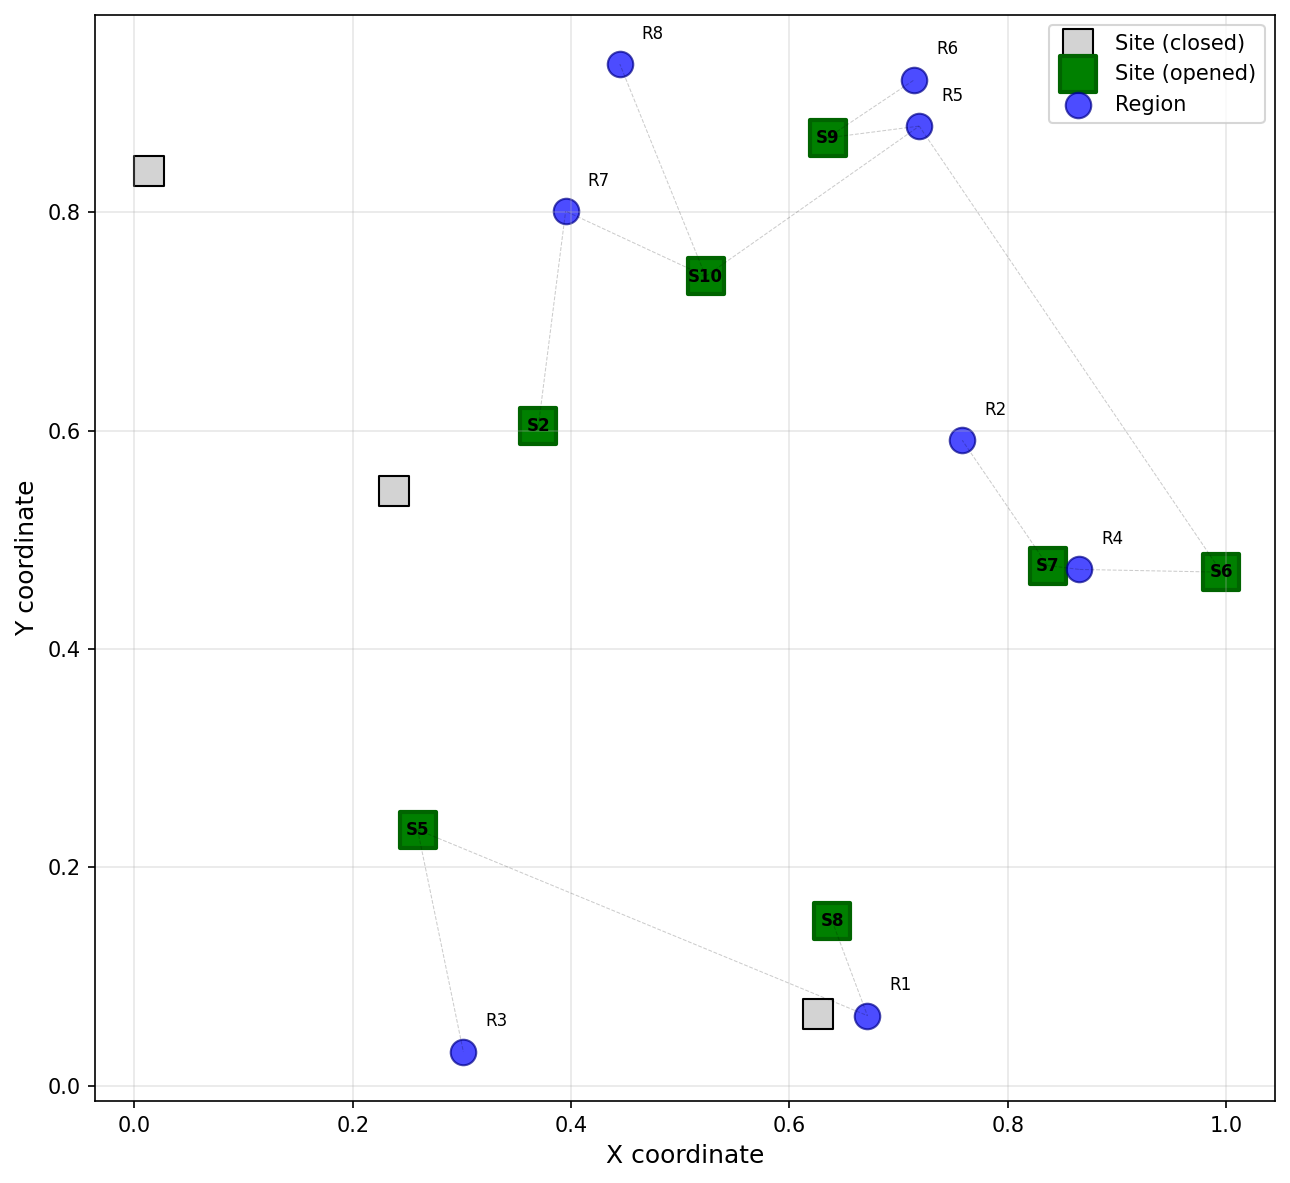
\includegraphics[width=0.48\textwidth]{fig/fig_map.png}\hfill
  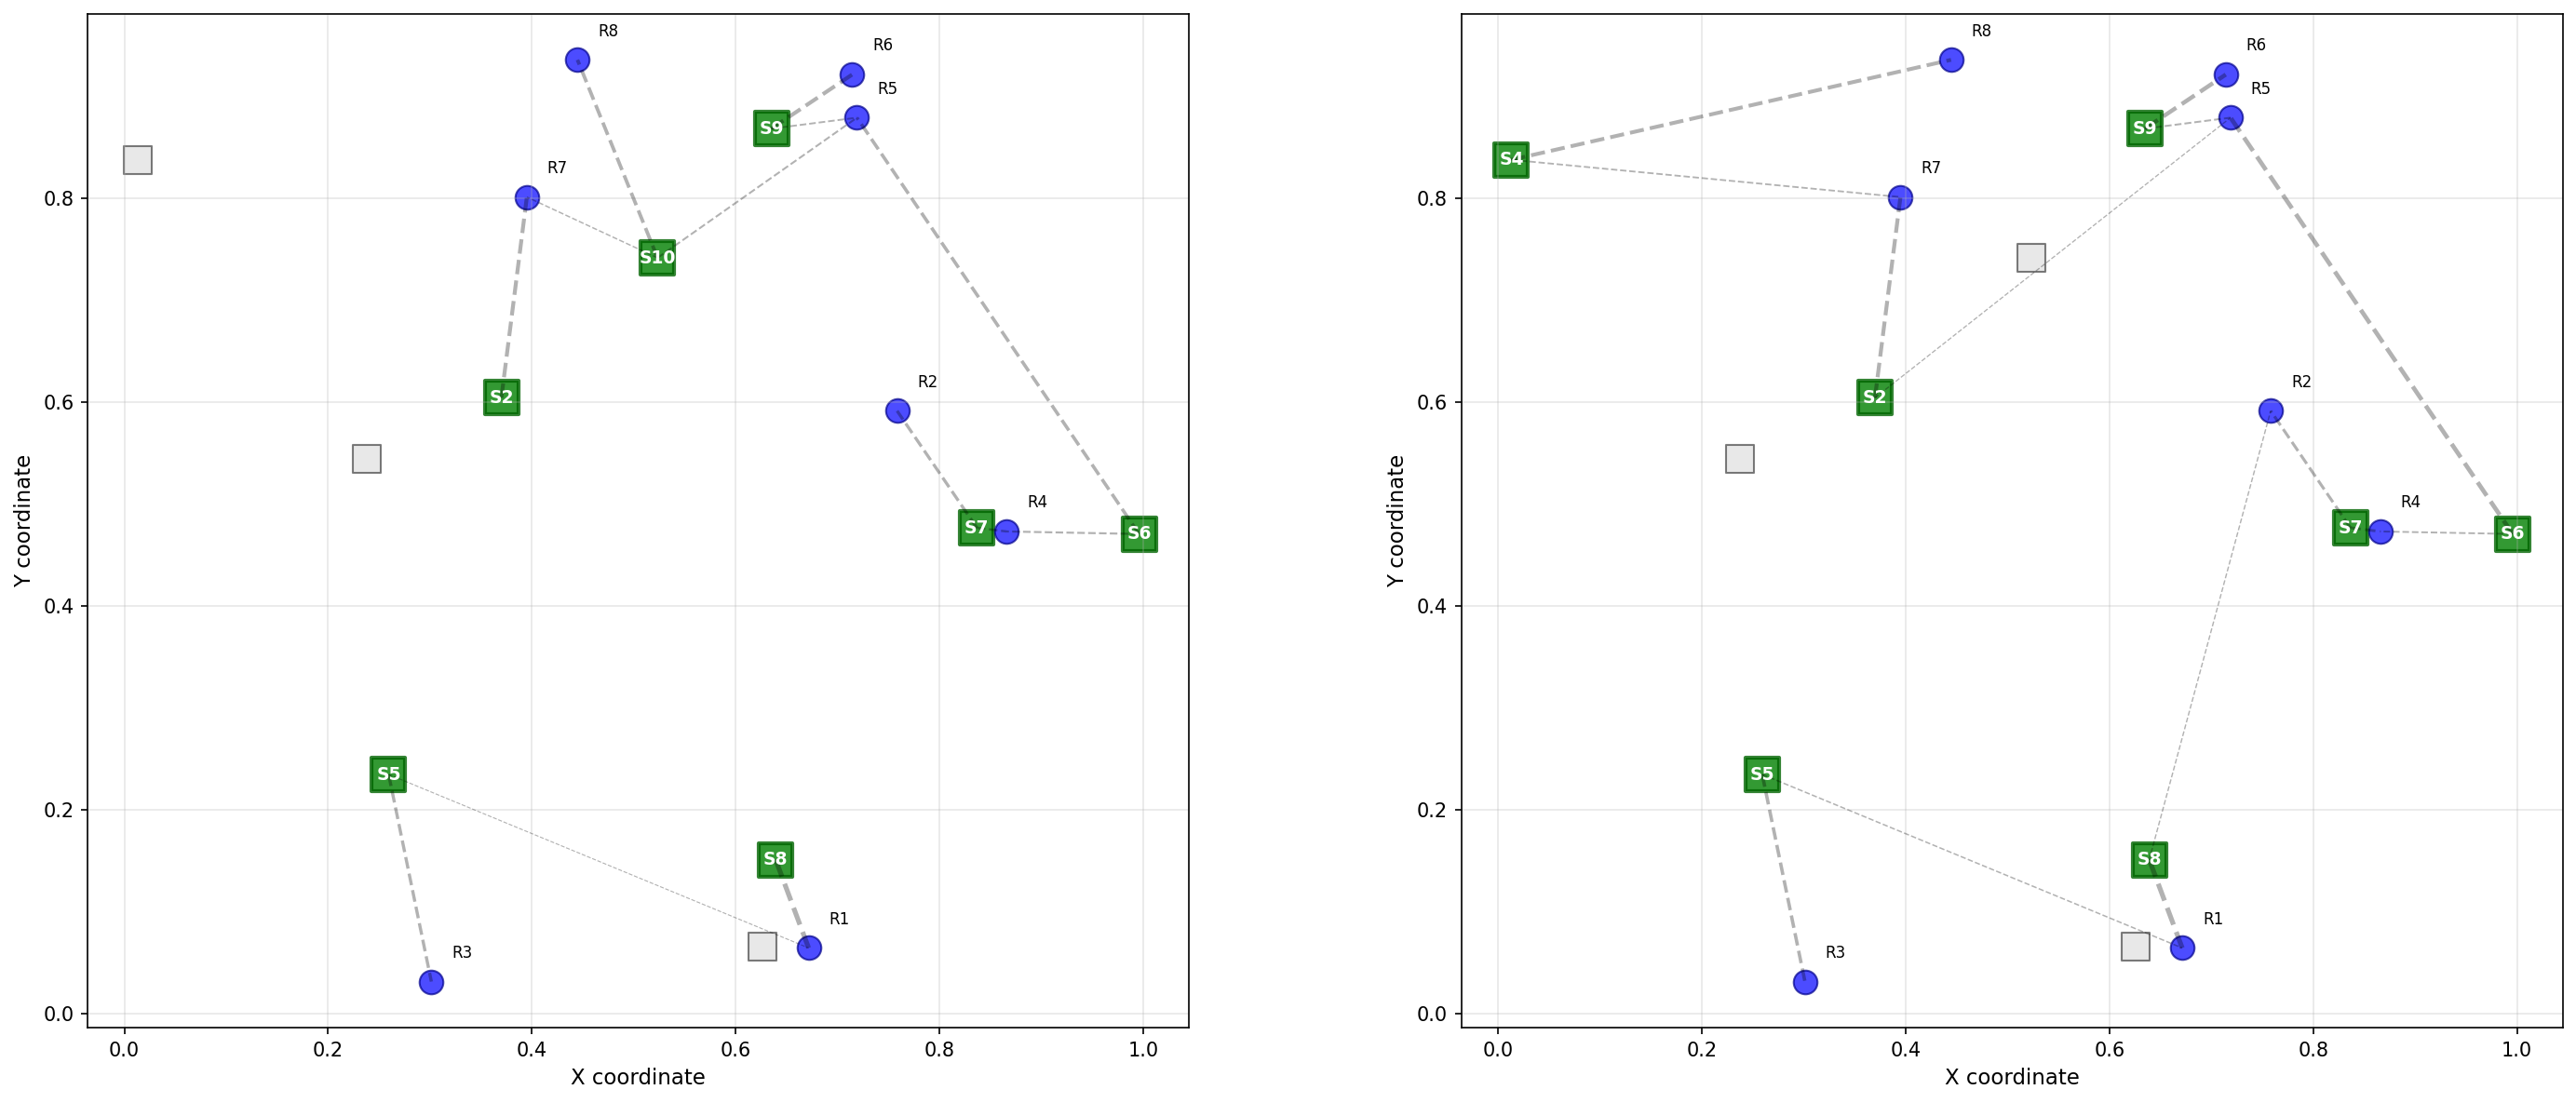
\includegraphics[width=0.48\textwidth]{fig/fig_side_by_side_maps.png}
  \caption{Toy geography and siting choices. Left: baseline siting and flows. Right: baseline (left panel) vs sustainability-aware (right panel) maps.}
  \label{fig:maps}
\end{figure}

\begin{figure}[t]
  \centering
  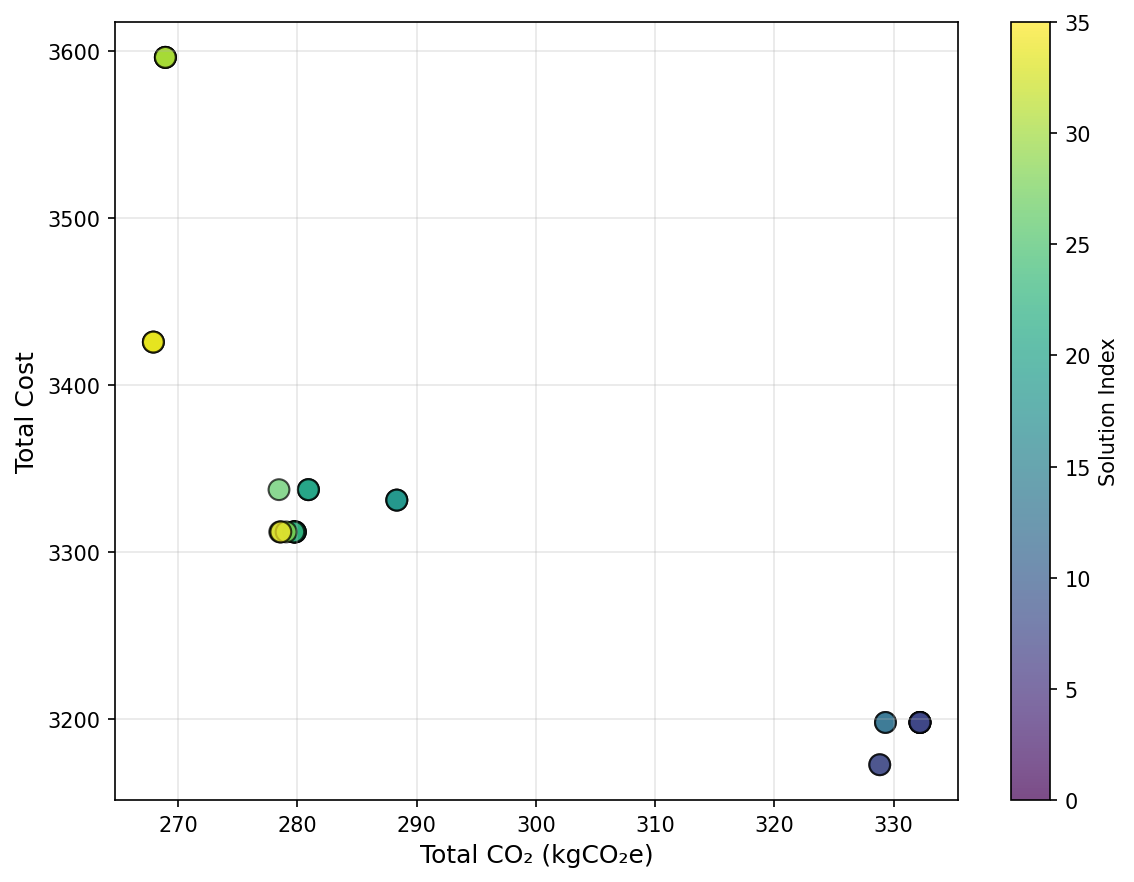
\includegraphics[width=0.48\textwidth]{fig/fig_tradeoff_cost_co2.png}\hfill
  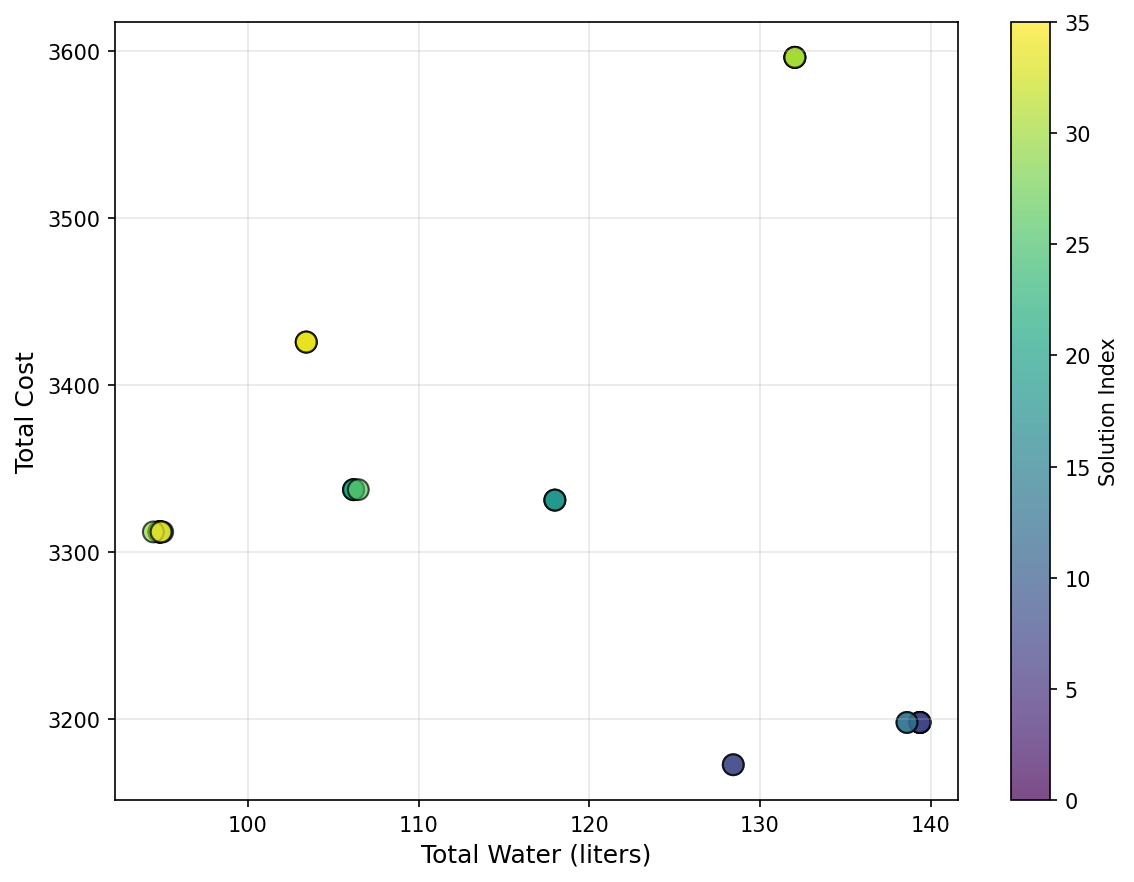
\includegraphics[width=0.48\textwidth]{fig/fig_tradeoff_cost_water.png}
  \caption{Cost–impact trade-offs from scalarized runs ($\lambda_{\mathrm{C}},\lambda_{\mathrm{W}}\in\{0,1,5,10,25,50\}$).}
  \label{fig:tradeoffs}
\end{figure}

\begin{figure}[t]
  \centering
  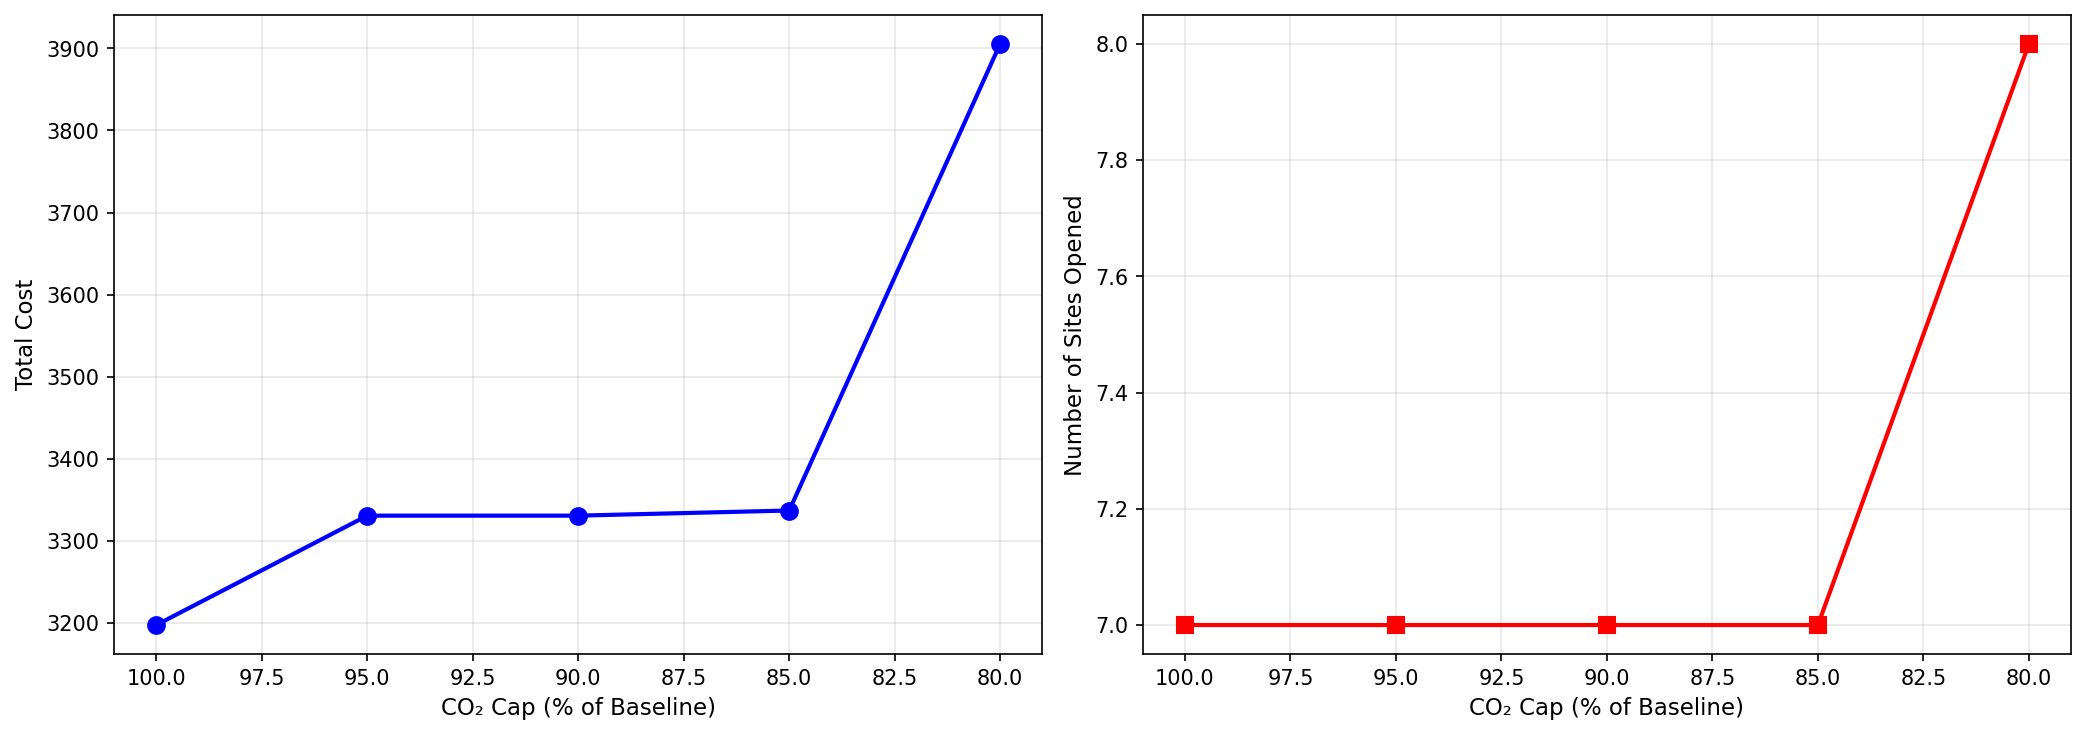
\includegraphics[width=0.7\textwidth]{fig/fig_sensitivity.png}
  \caption{Sensitivity to sustainability caps (percentage of baseline CO$_2$/water). Tightening caps raises cost and prompts site substitutions.}
  \label{fig:sensitivity}
\end{figure}

\paragraph{Reproducibility.} All experiments are scripted. Running \texttt{scripts/run\_all.py} reproduces the baseline, capped-impact, and scalarized runs and generates figures; \texttt{scripts/run\_sensitivity.py} tightens caps; \texttt{scripts/generate\_tables.py} exports Tables~\ref{tab:instance}--\ref{tab:siteshifts}. Generated assets live in \texttt{results/} and are copied to \texttt{latex/fig} for inclusion.

\section{Conclusion}\label{sec:conclusion}

We propose an Operations Research agenda for sustainable cloud operations, centered on a planning matrix that structures decisions across time horizons and operational stages. The matrix links managerial concerns to guiding questions, representative OR models, and sustainability levers, providing a consistent pathway from problem framing to tractable formulations. The Land \& Building Strategy application shows how a classical facility location model can be extended with carbon, water, and efficiency considerations without compromising tractability.

The main insight is that sustainability can be embedded directly into established optimization models through linear extensions, enabling cloud operators to quantify trade-offs among cost, performance, and environmental impacts. For researchers, the framework highlights opportunities where OR methods remain underexplored in cloud contexts—particularly at tactical and real-time horizons. For practitioners, it offers a scaffold to align operational efficiency and environmental stewardship within a single decision-support approach.

Future research should focus on the development of hybrid approaches that integrate optimization, simulation, and control, as well as the advancement of robust and stochastic formulations to address uncertainty. Fostering collaboration between academia and industry and constructing open datasets with sustainability metadata will be indispensable for guaranteeing that methodological advancements are translated into tangible outcomes. 

For practice, we recommend translating sustainability goals into model-ready parameters (e.g., caps, thresholds, internal prices), adopting standardized metrics for carbon, water, and reliability at both site and usage levels, and deploying decision-support tools that clearly communicate trade-offs and sensitivities to technical and non-technical stakeholders.

Sustainable cloud operations require decisions that render trade-offs explicit and hold outcomes accountable to measurable goals. The planning matrix and the decision-to-model procedure offer a unifying structure to make such decisions analyzable and optimizable, and we hope this agenda accelerates both methodological progress and real-world impact on the sustainability of cloud infrastructure.


\backmatter

\bmhead{Acknowledgements}
This work is supported by the “FrugalCloud” — INRIA and OVHCLOUD partnership.

\section*{Declarations}
\textit{to check if it needs to be filled.}

% Bibliography: use your sn-bibliography.bib with curated references (≈12–18)
\bibliography{sn-bibliography}

\end{document}
